\documentclass[10pt,a4paper]{article}
\usepackage[latin1]{inputenc}
\usepackage{amsmath}
\usepackage{amsfonts}
\usepackage{amssymb}
\usepackage{graphicx}
\usepackage{fancyhdr}
\usepackage{xcolor}
\usepackage{tikz}
\usepackage{enumerate}
\usetikzlibrary{arrows}
\title{Algebra 1 Mitschrift}


\author{JJS}

\definecolor{secback}{rgb}{0.75,0.75,0.75}
\definecolor{headerback}{rgb}{0.8,0.8,0.8}


%\renewcommand{\section}[1]{\refstepcounter{section}\setcounter{header}{0}\addcontentsline{toc}{section}{\thesection. #1}$\!$\vspace{0.3cm}\newline\vspace{0.01cm}\noindent\colorbox{secback}{\parbox{177.9mm}{\begin{LARGE}\textsc{\thesection. #1}\label{sec:\thepart\thesection}\end{LARGE}}}\vspace{0.3cm}\\}
%
%\newcommand{\header}[2]{\refstepcounter{header}$\!$\vspace{0.3cm}\newline\vspace{0.01cm}\noindent\colorbox{headerback}{\parbox{177.9mm}{\textbf{\theheader) #1} #2}}\vspace{0.3cm}\\}
%
%\newcommand{\headera}[2]{$\!$\vspace{0.3cm}\\\noindent\textbf{#1} #2\vspace{0.05cm}\hrule\vspace{0.3cm}\noindent}
%
%\usepackage[nohead,nofoot,lmargin=1.5cm,rmargin=1.5cm,tmargin=1.5cm,bmargin=1.5cm,headsep=0.5cm,headheight=12.4pt, foot=0.75cm]{geometry}
%\renewcommand{\footrulewidth}{0.4pt}
%\newcounter{header}


\usepackage[nohead,nofoot,lmargin=1.5cm,rmargin=1.5cm,tmargin=1.5cm,bmargin=1.5cm,headsep=0.5cm,headheight=12.4pt, foot=0.75cm]{geometry}
\renewcommand{\footrulewidth}{0.4pt}

%git
\pagestyle{fancy}
\fancyhf{}
\rhead{Seite \thepage}
\lhead{Optimierung 1 Mitschrift}
\lfoot{WS 08/09}
\cfoot{Jan Sommer}
\rfoot{sommerj@in.tum.de}
\setcounter{section}{-1}
\newcounter{def}
\setcounter{section}{4}
\begin{document}
%\maketitle
%\pagebreak
\hfill\textbf{14.10.2008}
\section*{Wiederholung}
\subsection*{Lineare Programme}
\[\max c^Tx\qquad,\qquad Ax\leq b\]
\subsection*{Polyeder}
Polyeder ist zul�ssiger Bereich eines LP
\begin{itemize}
\item $\mathcal H$-Darstellung (\textit{half-spaces}): $P=\left\{x\in\mathbb R^n\::\:Ax\leq b\right\}$
\item $\mathcal V$-Darstellung (\textit{vertex}): $P=conv(V)+pos(S)$ ($V$, $S$ endlich)
\end{itemize}
\subsection*{Kegel}
\begin{itemize}
\item $N_P(x^*)=\left\{c\in\mathbb R^n\::\:\max_{x\in P}c^Tx=c^Tx^*\right\}$
\item $S_P(x^*)=\bigcap_{c\in N_P(x^*)}H^{\leq}_{(c,0)}$
\item $S_P(B)=\left\{x\in\mathbb R^n\::\:A_Bx\leq0\right\}$
\end{itemize}
\subsection*{Simplexalgorithmus}
\begin{itemize}
\item Starte bei beliebiger Ecke
\item Bestimme Kanten von $S_P(B)$
\item Bestimme Verbesserungskante ($-A_B^{-1}$)
\item Laufe Verbesserungskante entlang zur n�chsten Ecke
\item[$\Rightarrow$] endliche, exponentielle worst case Laufzeit
\end{itemize}
\subsection*{Dualit�t}
Primales Problem (P):
\[\max c^Tx\qquad,\qquad Ax\leq b\]
Duales Problem (D):
\[\min b^Ty\qquad,\qquad A^Ty=c\:,\:y\geq0\]
Primale Nebenbedingung $\leftrightarrow$ duale Variablen
\subsection*{Komplementarit�t}
$x^*$ ist optimal f�r (P) genau dann, wenn $x^*$ zul�ssig ist und wenn es ein dual zul�ssiges $y^*$ gibt mit
\begin{itemize}
\item f�r alle $i$ mit $a_i^Tx^*<\beta_i$ $\Rightarrow$ $\eta^*_i=0$ oder
\item $c^Tx^*=b^Ty^*$ (starker Dualit�tssatz)
\end{itemize}
F�r zul�ssige $x$ und $y$ gilt (schwacher Dualit�tssatz):
\[c^Tx^*\leq b^Ty^*\]
\hfill\textbf{17.10.2008}
\section{Diskrete Strukturen}
\subsection{Graphen}
\subsubsection{Beispiel: Stra�enkreuzung}
\begin{itemize}
\item K�rzester Weg
\item Stra�enreinigung
\item TSP\\[1ex]
$\vdots$
\end{itemize}
\subsubsection{Bezeichung}
Sei $X$ eine Menge. Dann bezeichnet $2^X$ die \textit{Potenzmenge} von $X$. F�r $k\in\mathbb N$ sei
\[\binom Xk:=\left\{S\in2^X\::\:\vert S\vert=k\right\}\]
Menge der $k$-elementigen Teilmengen von $X$.
\subsubsection{Definition}
Seien $V$, $E$ endliche Mengen mit $V\cap E=\emptyset$ und $\nu:E\rightarrow\binom V1\cup\binom V2\cup V^2$. Dann hei�t $G:=(V,E,\nu)$ \textit{allgemeiner Graph}. Elemente von $V$: \textit{Knoten}, Elemente von $E$: \textit{Kanten}.\\[1ex]
Sei $e\in E$. Existiert ein $v\in V$ mit $\nu(e)\in\left\{\{v\},(v,v)\right\}$, so hei�t $e$ \textit{Schlinge}. Ist $\nu(e)\in\binom V1\cup\binom V2$, so hei�t $e$ \textit{ungerichtet}. Ist $\nu(e)\in V^2$, so hei�t $e$ \textit{gerichtet}. Gilt $\nu(e)=(v,w)$, so hei�t $v$ \textit{Anfangs-} und $w$ \textit{Endknoten} von $e$.\\[1ex]
Der allgemeine Graph $G$ hei�t \textit{schlingenfrei}, wenn $E$ keine Schlinge enth�lt. Sind alle Kanten ungerichtet bzw. gerichtet, dann hei�t $G$ \textit{ungerichtet} bzw. \textit{gerichtet}.\\[1ex]
Allgemeine schlingenfreie ungerichtete Graphen hei�en \textit{Multigraphen}. Analog \textit{gerichtete Multigraphen}.\\[1ex]
Ist $\nu$ injektiv und gibt es keine $e_1,e_2\in E$ und $v\in V$ mit  $\nu(e_1)=\{v\}$, $\nu(e_2)=(v,v)$, so hei�t $G$ \textit{schlicht} (\textit{einfach}).\\[1ex]
Sind $G(V,E,\nu)$ allgemeiner Graph, $\Phi:E\rightarrow\mathbb R$, so hei�t $(G;\Phi)$ \textit{gewichteter} allgemeiner Graph. F�r $e\in E$ hei�t $\Phi(e)$ \textit{Gewicht} (Kosten, L�nge, Kapazit�t $\dots$) von $e$.
 \subsubsection{Beispiel}
$V=\{v_1,v_2,v_3,v_4\}$, $E=\{e_1,\dots,e_8\}$ mit $V\cap E=\emptyset$, $v:E\rightarrow\binom V1\cup\binom V2\cup V^2$ definiert durch
\begin{align*}
\nu(e_1)&:=\{v_1\}\\
\nu(e_2)&:=(v_1,v_2)\\
\nu(e_3)&:=(v_2,v_1)\\
\nu(e_4)&:=\{v_1,v_4\}\\
\nu(e_5)&:=(v_1,v_3)\\
\nu(e_6)&:=\{v_3,v_4\}\\
\nu(e_7)&:=\{v_3,v_4\}\\
\nu(e_8)&:=(v_3,v_4)\\
\end{align*}
\paragraph*{Graphische Darstellung}
\begin{center}
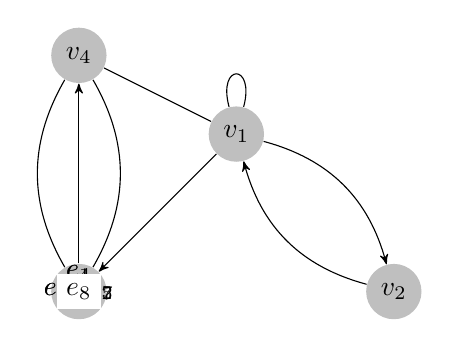
\begin{tikzpicture}[>=stealth']
\tikzstyle{vertex}=[circle,fill=black!25,minimum size=20pt,inner sep=0pt]
\tikzstyle{edge}=[draw,-]
\tikzstyle{arrow}=[edge,->]
\tikzstyle{every loop}=[]
\foreach \pos/\name in {{(2,2)/v_1},{(4,0)/v_2},{(0,0)/v_3},{(0,3)/v_4}}
  \node[vertex] (\name) at \pos {$\name$};
\path[edge,loop above] (v_1) to (v_1) node [midway] {$e_1$};
\path[arrow,bend left] (v_1) to (v_2) node [midway,right] {$e_2$};
\path[arrow,bend left] (v_2) to (v_1) node [midway,left] {$e_3$};
\path[edge] (v_1) to (v_4) node[midway,above] {$e_4$};
\path[arrow] (v_1) to (v_3) node[midway, right] {$e_5$};
\path[edge,bend left] (v_3) to (v_4) node[midway,left] {$e_6$};
\path[edge,bend left] (v_4) to (v_3) node[midway,right] {$e_7$};
\path[arrow] (v_3) to (v_4) node[midway,fill=white] {$e_8$};
\end{tikzpicture}
\end{center}
\subsubsection{Bezeichnung}
Seien $X$ eine nichtleere endliche Menge, $k:=\vert X\vert$. Jede Bijektion $\tau:\{1,\dots,k\}\rightarrow X$ hei�t \textit{Ordnung} (\textit{Reihenfolge}) auf $X$. Ist $\tau$ Reihenfolge auf $X$, so setzt man oft $x_i:=\tau(i)$ und schreibt $x=\{x_0,\dots,x_k\}$. Umgekehrt $\tau(i)=x_i$ legt Reiehenfolge fest.
\subsubsection{Definition}
Seien $G=(V,E,\nu)$ allgemeiner Graph, $n=\vert V\vert$, $m=\vert E\vert$, $m,n\geq1$
\begin{enumerate}[a)]
\item Seien $\tau_V,\tau_E$ Reihenfolgen auf $V$ bzw. $E$, dh. $V=\{v_1,\dots,v_n\}$, $E=\{e_1,\dots,e_m\}$. Ferner sei die $n\times m$-Matrix $S_G:=S_G(\tau_V,\tau_E):=\left(\sigma_{ij}\right)_{\underset{j=1,\dots,m}{i=1,\dots, n}}$ definiert durch
\[\sigma_{ij}:=\begin{cases}1&\text{falls }e_j\text{ ungerichtet und }v_i\in\nu(e_j)\\
-1&\text{falls }e_j\text{ gerichtet und }v_i\text{ Anfangsknoten von }e_j\\
+1&\text{falls }e_j\text{ gerichtet und }v_i\text{ Endknoten von }e_j\\
0&\text{sonst}\end{cases}\]
$S_G$ hei�t (\textit{Knoten-Kanten}) \textit{Inzidenzmatrix} von $G$. Der $j$-te Spaltenvektor von $S_G$ hei�t \textit{Inzidenzvektor} von $e_j$.
\end{enumerate}
\end{document}
